

\begin{center}
{\Large Билеты к коллоквиуму по матану 1 курс, 1 модуль}\\
\textbf{ЦПМ}\\ %You should put your name here
2018/19 учебный год %You should write the date here.
\end{center}

%\vspace{0.2 cm}

%1 done
\section{Вещественные числа, натуральные числа — определения. Аксиома Архимеда.}

На множестве $G$ определена \textit{бинарная операция}: каждой паре $(a,b), a \in G,b \in G$ элементов множества $G$ сопоставлен единственный элемент, обозначаемый $a*b$. Символом $*$ обозначается бинарная операция.

Множество $G$ называется \textit{группой} относительно операции $*$, если выполены следующие свойства:

    1.	Существует нейтральный элемент $e$, такой, что $\forall x \in G$ справедливо $x\cdot e = e\cdot x = x$
    
    2.	Существует обратный элемеакой, что $\forall x \in G \:  \exists y \in G$ такой что $x\cdot y = y\cdot x = e$
    
    3.	Операция $*$ ассоциативна: всегда $(a\cdot b)\cdot c =  a\cdot(b\cdot c)$
    
    4.	Операция $*$ коммутативна: всегда $a\cdot b = b\cdot a$

\underline{Аксиомы операций}

В множестве вещественных чисел заданы 2 коммутативных бинарных операции, сложения
и умножения.

1. Множество вещественных чисел $\bb{R} $ — аддитивная коммутативная группа.

2. Множество вещественных чисел $ \bb{R} \backslash  {0}$ — мультипликативная коммутативная группа.

3. Умножение дистрибутивно относительно сложения:$\forall x,y,z \in \bb{R}: (x+y)z = xz + yz$

Если выполнены такие аксиомы, то множество называется \textit{полем}.
Таким образом, первая аксиома вещественных чисел: на $\bb{R}$ заданы 2 операции, относительно
которых $\bb{R}$  является полем.

\textit{Поле} — это как раз множество, на котором есть 2 коммутативных операции,
связанные дистрибутивным законом.

\underline{Аксиомы порядка}

Мы будем говорить, что на множестве $A$ определено отношение $\leq$, если в множестве пар $(a,b),a \in A,b \in A$ выбрано некоторое подмножество. Если пара $(a,b)$ принадлежит  подмножеству, то будем говорить, что $a \leq b$.

Отношение называется \textit{отношением порядка}, если выполнены следующие свойства:

1. $a \leq a$;

2. $(a \leq b) \wedge (b \leq a) \Rightarrow a = b$;

3. $(a \leq b) \wedge (b \leq c) \Rightarrow a \leq c$;

4. $\forall a,b \in A$ либо $a \leq b$, либо $b \leq a$.

Если выполнено свойство 4, то множество называется \textit{линейно упорядоченным}, если нет - \textit{частично упорядоченным}.

\textit{Поле $F$ называется упорядоченным полем, если на этом поле задано отношение порядка, $F$ линейно упорядочено, причём $a \leq b\: \Rightarrow \: a + c \leq b + c$ при любом $c \in F$ и $(0 \leq a) \wedge (0 \leq b) \Rightarrow 0 \leq ab$.}

\underline{Аксиома непрерывности}

Пусть $A,B \subset \bb{R}, A,B \neq \varnothing$
 причём $\forall a \in A, b \in B$ справедливо $a \leq b$. Тогда существуетт такое $c \in \bb{R}$, что $\forall a \in A$ справедливо $a \leq c$, и $\forall b \in B$ справедливо  $c \leq b$.

\underline{\textit{ОСНОВНОЕ ОПРЕДЕЛЕНИЕ:}}
\begin{center}
    \textbf{Множеством вещественных чисел} называется упорядоченное поле с аксиомой непрерывности.
\end{center}


\underline{Аксимома Архимеда}

\textit{Для любых вещественных чисел $a, b > 0 $ среди чисел
$a, a + a(= 2a), a + a + a(= 3a), . . . , na, . . .$ найдутся числа, большие чем $b$}

$\blacktriangleleft$  \text{Рассмотрим множество } $A$ \text{ таких чисел вида} $ n*a$. \text{ Допустим, что среди них нет ни одного числа, большего } $b$.\\
\text{ Рассмотрим множество } $B$ \text{ вещественных чисел, больших всех чисел из} $ A$. \text{ Множества } $ A$ \text{и} $ B$ \text{ не пустые } $(b \in B)$. \text{ Все элементы множества} $A$ \text{меньше всех элементов} $B$ $\Rightarrow \text{по аксиоме непрерывности между}$  $A $ \text{и} $ B $ \text{найдется промежуточное число} $ \alpha $:
		\begin{align}
		x \leq \alpha \leq y,& x \in A, y \in B.
		\end{align}
Это число $ \alpha $ по построению — точная верхняя грань$ A, \alpha = sup A. $
Однако,  $ \beta = \alpha-a \in B  $ по построению $ (\alpha > a+. . .+a $ при любом количестве слагаемых, значит,
$ \beta > a + . . . + a $ также при любом их количестве), а это противоречит $\alpha = sup A $. $\blacktriangleright$

\underline{Аксиома Архимеда уточненная}

\textit{Для любого $h > 0$ и для любого $a \in \bb{R}$ найдется такое $n \in \bb{Z}$, что справедливы неравенства $(n - 1)h \leq a < nh$.}

$\blacktriangleleft$ 
\text{Рассмотрим множество}  $\: E = {n \in \bb{Z}}$.
\text{Множество} $E$ \text{не пусто и огарничено снизу: если} \\
$a > 0$, 
\text{то не пуcто по аксиоме Архимеда, ограничено снизу нулем; если} $a < 0$,\\ \text{то не пусто так как содержит ноль, ограничено по аксиоме Архимеда.}\\
Пусть $m = min \: E$. Тогда $m - 1 \leq a/h < m$, отсюда следует учточнённая аксиома Архимеда. $\blacktriangleright$




\underline{Множество натуральных чисел N} — это пересечение всех индуктивных*
 подмножеств $\bb{R}$, содержащих 1.

Множество$  X \subset R $ называется индуктивным, если $ \forall x \in X : x + 1 \in X $.\\
Примеры: $ \mathbb{R},\mathbb{Z}, \mathbb{Q}, \mathbb{R}
 \backslash \mathbb{Q}$\\
Пересечение $ X = \cap X_{\alpha} $ любого
 набора индуктивных множеств или пусто, или само является
индуктивным множеством. В самом деле: $ x \in X \Rightarrow \forall \alpha : x \in X\alpha\Rightarrow \forall \alpha : (x+1) \in X_{\alpha} \Rightarrow (x+1) \in  X $
\\\\
 Из определения следует принцип математической индукции: если $ E \subset N, 1 \in E $ и $ E $ —
 индуктивное множество, то $ E = N $.
 Эта формулировка эквивалентна более привычной: если какое-то утверждение верно для
 $ n = 1 $ и если из того, что оно верно для натуральных чисел $ n \leqslant k $ следует, что оно верно для
 $ n = k + 1 $, то это утверждение верно для всех натуральных чисел.
 Чтобы увидеть эту эквивалентность, достаточно обозначить множество, для которого верно
 утверждение, буквой $  E $, вывод $ E = N $ означает, что утверждение верно для всех $  n $.
 
 Свойства натуральных чисел:
 
 1. Сумма и произведение натуральных чисел - натуральное число;
 
 2. $\forall n \in \bb{N}, n \neq 1: n - 1 \in \bb{N}$;
 
 3. $\forall n \in \bb{N}: min{x \in \bb{N}: x > n} = n + 1$
 
 4. $\forall n \in \bb{N}: {x \in \bb{N}: n < x < n + 1} = \varnothing$;
 
 \underline{Теорема.}\textit{ Множество $\bb{N}$ вполне упорядоченo.}
 
 $\blacktriangleleft$ Пусть $M \subset \bb{N}$. Если $1 = min M$. Если $1 \notin M$, то есть $1 \in E=\bb{N}\backslash M$. В множестве $E$ найдется такое $n$, что $1,...,n \in E, (n + 1) \in M$. Если бы такого $n$ ненашлось бы, то $E$ было бы индуктивным множеством и совпадало бы с $\bb{N}$. Но тогда $M = \bb{N} \backslash E = \varnothing$, что не так по предположению. 
 Найденное число $n + 1 \in M$ и есть минимальный элемент в $M$. $\blacktriangleright$
 \\
 \\
 

%2 done
\section{Ограниченные множества, точная верхняя грань.}

Множество $A \subset \bb{R}$ называется \textit{ограниченным сверху}, если существует такое число $M \in \bb{R}$,что для любого $x \in A$ справедливо $x \leq M$. Число $M$ называется \textit{верхней границей} множества $A$.

Множество ограничено сверху $\Leftrightarrow$ у множества есть верхняя граница.

Подмножество $A \subset \bb{R}$ называется \textit{ограниченным снизу}, если сущесвует такое число $m \in \bb{R}$, что для любого $x \in A$ справедливо $x \geq m$.
Число $m$ называется \textit{нижней границей} множества $A$.

Подмножество $A \subset \bb{R}$ называется \textit{ограниченным}, если оно ограничено сверху и снизу.

\textit{Число $M \in A$ называется максимальным или наибольшим элементом множества $A$,если оно является верхней границей множества $A$, то есть для любого $x \in A$ справедливо $x \geq m$.} Из аксиомы порядка следует единственность максимума и минимума любого множества из вещественных чисел, если этот минимум или максимум существует.

Рассмотрим множество $A^+$ всех границ множества $A$. Наименьший элемент множества $A^+$ называется \textit{точная верхняя грань} множества $A$ и обозначается $sup A$. Аналогично определяется \textit{точная нижняя грань $A$} и обозначается $inf A$.

\underline{Теорема} \textit{У любого непустого ограниченного сверху множества $A$ существует точная верхняя грань.}

$\blacktriangleleft$  Пусть $A^+$ - множество верхних границ множества $A$. Оба множества $A$ и $A^+$ не пустые и выполнено условие аксиомы непрерывности: все элементы первого множества не больше всех элементов второго множества $\Rightarrow$ существует $M$ такое, что $\forall x \in A, y \in A^+: x \leq M \leq y$.

По построению, $M = sup A$: число $M$ является верхней границей, так как $\forall y \in A^+: y \geq M$. $\blacktriangleright$

Аналогично, у любого ограниченного снизу множества $A \neq \varnothing$ существует точная нижняя гарнь и она единственная.
        
\textit{Упорядоченное поле, в котором каждое ограниченное сверху множество имеет точную верхнюю грань, есть $\R$.}
\\
\\



%3 done
\section{Теорема о вложенных промежутках.}

\textit{Любая последовательность вложенных отрезков $\Delta_n = [a_n, b_n]$ имеет непустое пересечение. Если их длины $b_n - a_n$ стремятся к нулю, то это пересечение $\bigcap_{n=1}^\infty \Delta_n$ состоит из единственной точки.}

Рассмотрим два множества: множество $A$, состоящее из точек $a_n$ (левых концов отрезков) и множество $B$, состоящее из точек $b_n$ (правых концов отрезков). Заметим, что какое-то из этих множеств вполне может оказаться конечным.

Множества $A$ и $B$ удовлетворяют условиям аксиомы непрерывности (они не пустые и каждое $a_m$ не превосходит каждого $b_n$), поэтому существует число $\gamma \colon a_m \leq \gamma \leq b_n$ при всех $m,n \in \bb{N}$. Отсюда следует искомое включение $\gamma \in \cap_{n=1}^\infty \Delta_n$.

Единственность точки $\gamma$ следует из $b_n - a_n \rightarrow 0$. Если бы было 2 таких различных точки $\gamma_1 < \gamma_2$, то из неравенств $a_n \leqslant \gamma_1 < \gamma_2 \leqslant b_n$ следовало бы неравенство $b_n - a_n > \ep = \gamma_2 - \gamma_1 > 0$, которое противоречит $b_n - a_n \rightarrow 0$.
\\
\\


%4 done
\section{Предельные и граничные точки. Множество предельных точек -- замкнуто.}

\textbf{Предельная точка} $x$ - предельная точка $X$,  $x \in X \{\forall\varepsilon \; \exists y \in X\; |x-y|<\varepsilon\}  $\\
\textbf{Граничная точка} $x$ - граничная точка $X$,  $ x \in X \{ \forall\varepsilon \; \exists y \in X  \; \exists c\notin X\;|x-y|<\varepsilon \wedge |x-c|<\varepsilon\}  $\\
\textit{Множество $A'$ предельных точек множества $A$ замкнутое.}\\
$\blacktriangleleft$
Пусть $A'$ - множество предельных точек множества $A$. Пусть $x$ - предельная точка множества $A$. Тогда в любой окрестности $O(x)$ точки $x$ лежит точка $y \in A'$, предельная точка множества $A$. Возьмем окрестность $O(y)$ точки $y$, целиком лежащую в $O(x)$ и не содержащую $x$. По определению предельной точки там лежит точка $z \in A.$ Эта точка лежит в $O(x)$ и не совпадает с $x$. \\
Мы доказали, что в любой окрестности точки $x$(предельной для $A'$) лежит точка $y \neq x, y \in A.$ Значит, $x \in A'$. Итак, каждая предельная точка множества $A'$ ему принадлежит, множество $A'$ - замкнутое.$\blacktriangleright$


%5 done
\section{Открытые и замкнутые множества. Дополнение к замкнутому множеству
-- открытое и наоборот.}

\textbf{Открытые множества} -- множество называется открытым, если оно не имеет граничных точек.  Иными словами множество $X$ называется открытым если $\forall x_{0}\in X\{\forall x \in X  \;\exists\varepsilon \; |x-x_{0}|<\varepsilon \} $. Если все его точки внутренние(если найдется окрестность точки, целиком лежащая в множестве).\\
\textbf{Замкнутое множества} - множество называется замкнутым, если оно содержит все свои предельные точки.  Иными словами множество $X$ называется замкнутым если $  \nexists x \notin X \{\forall\varepsilon \; \exists y \in X\; |x-y|<\varepsilon\}  $\\
\textbf{Теорема. Пусть $ A $ — открытое множество, $ B $ — замкнутое множество. Тогда 1) $ A \backslash B $
	— открытое множество. 2) $ B \backslash A  $— замкнутое множество}\\
1)Обозначим как $ X_{P} $ как множество всех предельных точек множества $ P $ .

\begin{equation*}
    x \in  A \backslash B  \Leftrightarrow x \in  A \wedge x \notin  B 
    \leqno(1)
\end{equation*}
\begin{equation*}
   x \in  A \wedge x \notin  B \Rightarrow  \forall x_{B} \in X_{B}\; x_{B}\notin A \backslash B \text{ Т.к. B - закрытое множество}
    \leqno(2)
\end{equation*}
\begin{equation*}
   x \in  A \Rightarrow X_{ A \backslash B }\cap X_{A}=\emptyset
    \leqno(3)
\end{equation*}
\begin{equation*}
   \text{Из (3) и (4) } \Rightarrow X_{ A \backslash B } \subset X_{A}\Rightarrow  X_{ A \backslash B }\text{ - не содержит граничных точек}\Rightarrow A \backslash B  \text{ - открытое}
    \leqno(4)
\end{equation*}

Утверждение доказано.
2)Обозначим как $ X_{P} $ как множество всех предельных точек множества $ P $ .

\begin{align}
x \in  B \backslash A \Leftrightarrow x \in  B \wedge x \notin  A\\
x \in  B \wedge x \notin  A\Rightarrow  X_{ A \backslash B }\subset X_{B}\\
X_{ A \backslash B } \subset X_{B} \Rightarrow X_{ A \backslash B} \cap A=\emptyset(\text{ Т.к. B закрытое множество }) \;\;  X_{ A \backslash B} \subset B \Rightarrow X_{ A \backslash B} \subset A \backslash B \Rightarrow A \backslash B  \text{ - закрытое}
\end{align}
Утверждение доказано.
\\
\\

%6 done
\section{}

\textbf{Всякое ограниченное бесконечное множество имеет по крайней мере одну предельную точку.}

$\blacktriangleleft$
\text{Дано ограниченное бесконечное множество} $\: E$. \text{Пусть отрезок} $\: [a_1, b_1], b_1 > a_1$ содержит $E$. \\
Разделим отрезок $[a_1,b_1]$ пополам точкой $(a_1 + b_1)/2$ на 2 отрезка: $L_1 = [a_1, (a_1 + b_1)/2]$ и $R_1 = [(a_1 + b_1)/2, b_1]$.  По крайней мере одно из множеств $L_1 \cap E$ или $R_1 \cap E$ содержит бесконечное множество точек. Пусть, например, это будет множество $R_1 \cap E$. Обозначим отречок $R_1$ через $[a_2, b_2]$. \\ Разделим его пополам на отрезки и снова выберем множество, которое содержит бесконечное множество точек, повторим процедуру бесконечно много раз.\\
Мы получим последовательность вложенных отрезков $[a_n, b_n]$, длины этих отрезков равны \\ $(b_n - a_n) = (b_1 - a_1)2^{-n+1}\rightarrow 0$. Итак, персечение всех этих открезков состоит из единственной точки $\alpha$. Это есть предельная точка множества $E$: любая окрестность точки $\alpha$ содержит все отрезки $[a_n, b_n]$ с достаточно большими номерами, на каждом отрезке есть бесконечное количество точек множества $E$.\\
\\
\\





%7 done
\section{}

\textbf{Покрытия. Лемма Гейне–Бореля (компактность отрезка).}\\
Пусть дано множество $A$ и ещё дана система $U$ множеств $B_\alpha$, причём $A \subset \bigcup _\alpha B_\alpha$. Тогда говорят, что система $U$ образует \textit{покрытие} множества $A: \forall x \in A \: \exists B_\alpha : x \in B_\alpha$.\\
Любое подмножество системы $U$, если оно также является покрытием, называется \textit{подпокрытием}. Покрытие $U$ называют открытым, если все множества $B_\alpha \in U$ открытые. Покрытие $U$ называют конечным, если оно содержит конечное множество множеств $B_alpha$.\\
\underline{Лемма Гейне-Бореля.} \textit{Любое открытое покрытие} $\bigcup _\alpha I_\alpha$ \textit{отрезка} $\Delta $ \textit{ имеет конечное подпокрытие.}\\
$\blacktriangleleft$
\text{ Пусть отрезок } $\Delta = [a_1, b_1], b_1 > a_1$ \text{покрыт бесконечной системой открытых множеств} $I_\alpha : \Delta \subset \bigcup _\alpha I_\alpha$.
\text{Пусть не существует конечного подпокрытия, нельзя выбрать конечный набор } $I_{\alpha_k}, k = 1,2,...,N$ 
\text{ открытых множеств, также покрывающее открезок} $\Delta$.\\ \text{Разделим отрезок} $[a_1, b_1]$ \text{пополам точкой} $(a_1 + b_1)/2$ \text{ на 2 отрезка:} \\ $\: L_1 = [a_1, (a_1 + b_1)/2]$ и $R_1 = [(a_1 + b_1)/2, b_1].$ \\ 
\text{По крайней мере для одного из отрезков не существует конечное подпокрытие из покрытия } $I_\alpha$.\\
\text{Пусть, например, это отрезок } $R_1$. \\ 
\text{Разделим его пополам и для новых открезков проделаем то же самое, повторим этo бесконечно}\\ \text{много раз.}\\
Мы получим последовательность вложенных отрезков $[a_n, b_n]$, длины этих отрезков равны \\ $(b_n - a_n) = (b_1 - a_1)2^{-n+1}\rightarrow 0$. Эти отрезки строились так, чтобы ни один из них не мог быть покрыт конечным набором множества $I_\alpha$.\\
По лемме о вложенных отрезках пересечение всех этих отрезков сосотоит из единственной точки $\gamma$.\\
Эта точка $\gamma$ принадлежит какому-то открытому множеству $I$ из открытого покрытия. Вместе с точкой $\gamma$ открытое множество $I$ содержит и некоторую окрестность точки $\gamma$. Теперь, при достаточно больших $n$ отрезки $[a_n, b_n]$ все покрыты один единственнным открытым множеством $I$ из покрытия. Полученное противоречие доказывает лемму Гейне-Бореля. $\blacktriangleright$
\\ 
\text{Доказанная лемма означает, что отрезок(= замкнутый промежуток) - компакт.}
\\
\\



%8 done
\section{Нигде не плотные и всюду плотные множества. Теорема Бэра.}

Множество $A \subset [0,1]$ называется \textit{всюду плотным}, если замыкание $\overline{A}$ множества $A$ содержит $[0,1]$. Множество $A \subset [0,1]$ называется \textit{нигде не плотным}, если внутри любого интервала $U \subset [0,1]$ есть меньший интервал $V \subset U$ такой, что $A \cap V = \varnothing$.\\
Множество $A$ \textit{всюду плотно на } $[0,1]$, если внутри любого интервала $U \subset [0,1]$ есть точка из $A$. Иначе говоря, если $[0,1] \subset \overline{A}$. \\
\underline{Теормема Бэра.} \textit{Отрезок не может быть покрыт объединением счетного числа нигде не плотных множеств.}\\
$\blacktriangleleft$
\text{Пусть } $[0,1] \subset \bigcup_{n=1}^\infty A_n$, где все множества $A_n$ - нигде не плотные.
Тогда выберем отрезок, $\Delta _1 \subset [0,1]$, на котором нет точек из $A_1$, потом выберем отрезок, $\Delta _2 \subset \Delta _1$, на котором нет точек из $A_2$, и так далее. В опр нигде не плотного множества стоят интервалы, но это не страшно, будем выбирать интервалы, а потом в каждом из них выберем отрезок чуть поменьше. \\ Последовательность вложенных отрезков $\Delta _n$ имеет общую точку, эта точка не принадлежат ни одному из множеств $A_n \Rightarrow$ предположение не верное.
\\
\\

%9 done
\section{Компактность и секвенциальная компактность.}

\underline{Определение.} Множество называется компактным, если из любого его открытого покрытия можно извлечь конечное подпокрытие.\\
\underline{Определение.} Множество $E$ называется секвенциально компактным, если из любой последовательности $x_n \in E$ можно извлечь подпоследовательность, сходящуюся к пределу, лежащему в $E$.\\
\underline{Теорема.} Множество $E\in\bb{R}$ компактно, если и только если оно секвенциально компанктно.
\underline{Теорема.} Множество $E\in\bb{R}$ компактно, если и только если оно замкнуто и ограничено.\\
Доказательство по следующей схеме:\\
1)Если множество ограничено и замкнуто, то оно секвенциально компактно.\\
2)Если множество  ограничено и замкнуто, то оно компактно.\\
3)Если множество не ограничено, то оно не компактно и не секвенциально компактно.\\
4)Если множество не замкнуто, то оно не компактно и не секвенциально компактно.\\

$\blacktriangleleft$ 1) Из ограниченноц последовательности можно извлечь сходящуюся подпоследовательность, она принадлежит множеству, так как множество замкнуто, то и предел принадлежит множеству. $\blacktriangleright$\\
$\blacktriangleleft$ 2) Пусть есть ограниченное и замкнутое множество $E$ и его открытое покрытие  $\bigcup U_{\alpha}$. Множество $E$ принадлежит некоторому отрезку $[a,b]$. Множество $(a-1, b+1)\smallsetminus E$ - открытое. Рассмотрим покрытие отрезка $[a,b]$, состоящее из всех множеств $\bigcup U_{\alpha}$ и множества $(a-1,b+1)\smallsetminus E$. Каждая точка отрезка покрывается, точки из $E$ покрываются множествами из $\bigcup U_{\alpha}$, точки не из $E$ - точками из $(a-1,b+1)\smallsetminus E$. Теперь выберем по лемме Гейне-Бореля из покрытия $\bigcup U_{\alpha}\bigcup(a-1,b+1)\smallsetminus E$ отрезка $[a,b]$ конечное подпокрытие. Оно состоит из конечно симла множеств $\bigcup U_{\alpha}\colon \{U_{\alpha 1},...,U_{\alpha n}\} $  и множества $(a-1,b+1)\smallsetminus E$, которое с $E$ не пересекается. Поэтому $\{U_{\alpha 1},...,U_{\alpha n}\}$ - конечное покрытие $E$ $ \blacktriangleright$\\
$\blacktriangleleft$ 3) Пусть множество $E$ неограничено, например, сверху. Тогда есть последовательность $x_n \in E$,\ $x_n \rightarrow \infty$. Без потери общности можно считать последовательность $x_n$ монотонной. Из этой последовательности нельзя извлечь сходящуюся. Поэтому, $E$ не секвенциально компактно.$\blacktriangleright$\\
$\blacktriangleleft$ 4) Пусть множество $E$ ограничено, но не замкнуто. Это значит, что у него есть предельная точка $x^*$, которая не принадлежит множеству $E$.\\
По определению предельной точки выберем последовательность $x_n \in E$, сходящуюся к $x^*$. Любая ее подпоследовательность сходится к той же точке $x^*$, которая не принадлежит множеству $E$. Поэтому множество $E$ не секвенциально компактное.\\
Теперь построим открытое покрытие $E$, из которого нельзя выбрать конечное подпокрытие. Его легко выписать в явном виде, например, в него можно включить все лучи вида $(-\infty, x^*-\frac{1}{n})$ и все лучи $(x^*+\frac{1}{n}, +\infty)$. Это покрытие множества $\bb{R} \smallsetminus {x^*} \rightarrow$ покрытие $E$. Любая конечная система множеств из такого покрытия не содержит некоторую окрестность точки $x^*$, но по определению предельной точки в ней обязательно есть точки множества $E$, то есть эта конечная система не является покрытием.$\blacktriangleright$\\


%10 done
\section{Предел последовательности, сходимости к бесконечности — определения. Лемма о двух
милиционерах.}

\textit{Последовательность вещественных чисел} - функция с областью определения $\bb{N}$ и областью значений $\bb{R}$.\\
Число $A$ называется \textit{пределом последовтельности} $ x_n$ ($\lim _{n \rightarrow \infty} x_n = A$), если вне любой окрестности точки $A$ лежит лишь конечное множество элементов последовательности $x_n$, или, что то же самое, все элементы $x_n$ с достаточно большими номерами $n$ лежат внутри этой окрестности.\\
$ \lim _{n \rightarrow \infty} x_n = A \:  \Leftrightarrow \forall \epsilon > 0 \: \exists N \in \bb{N} \: \forall n > N: |x_n - A| < \epsilon$.\\
Если у последовтельности есть какой-то предел, то говорят, что такая последовательность сходится. \\
Последовательность не сходится \\ $\forall A \: \exists \epsilon > 0 \: \forall N \in \bb{N} \: \exists n > N: |x_n - A| > \epsilon$. \\
Последовательность не сходится к $A$ \\
$\exists \epsilon > 0 \: \forall N \in \bb{N} \: \exists n > N: |x_n - A| > \epsilon$.

\underline{Определение сходимости к бесконечности.} Будем говорить, что последовательность $x_n$ сходится к $+\infty$, если $\forall K \: \exists N \in \bb{N} \: \forall n > N: x_n > K.$ \\
\underline{Лемма о двух милиционерах}\\
Пусть даны 3 последовательности, причём $x_n \leq y_n \leq z_n$.\\
\textit{Пусть существуют пределы } $\lim _{n \rightarrow \infty} x_n =  \lim _{n \rightarrow \infty} z_n = A$. \textit{Тогда существует предел} $\lim _{n \rightarrow \infty} y_n$ \textit{и он также равен $A$}\\
$\blacktriangleleft$
$\lim _{n \rightarrow \infty} x_n = \lim _{n \rightarrow \infty} z_n = A:$\\
$\forall \epsilon > 0 \: \exists N \: \forall n > N: |x_n - A|, |z_n - A| < \epsilon.$\\
Это то же самое, что $ \forall \epsilon > 0 \: \exists N \: \forall n > N: A - \epsilon < x_n \leq z_n < A + \epsilon$.\\
$\forall \epsilon > 0 \: \exists N \: \forall n > N: A - \epsilon < y_n < A + \epsilon$.
$\blacktriangleright$
\\
\\


%11 done
\section{Подпоследовательности, выбор сходящейся подпоследовательности. Частичные пределы. Верхний предел,
нижний предел.}

\textit{Последовательность строго возрастает, если $x_n < x_{n+1}$ при $n \in \bb{N}$.}\\
\underline{Подпоследовательность}\\
Пусть у нас есть последовательность $x_n$. Предположим, задана строго возрастающая последовательность $n_k, k = 1,2,... \:$ с положительными целыми элементами. \\
Тогда можно рассмотреть композицию отображений $k \mapsto n_k, \: n \mapsto x_n$, ставящую в соответствие каждому натуральному числу $k$ элемент последовательности $x_{n_k}$.\\
Такая последовательность называетсяя подпоследовательностью последовательности $x_n$.
Последовательность $n_k$ должна быть монотонная.\\
Теорема. \textit{Если последовательность $x_n$ сходится, то и каждая подпоследовательность $x_{n_k}$ сходится к тому же пределу.}\\
Теорема. \textit{Если подпоследовательность $x_{n_k}$ содержит все элементы последовательности $x_n$ кроме конечного числа, то из сходимости подпоследовательности следует сходимость самой последовательности}\\
\underline{Теорема(лемма Больцано - Вейерштрасса).}
\textit{Всякая ограниченная последовательность $x_n \in \bb{R}$ имеет сходящуюся подпоследовательность}\\

$\blacktriangleleft$
\text{Так как элементов последовательности бесконечное (счётное) множество,} \\ \text{ то либо множество значений, которые принимают элементы последовательности, бесконечно,}\\ \text{либо какое-то из значений последовательность принимает бесконечное количество раз} \\ \text{(возможно, таких значений много).В этом случае можно выбрать постоянную подпоследовательность,} \\ \text{ которая сходится. Если же множество значений, которые принимают элементы последовательности,} \\ \text{ бесконечно, то воспользуемся теоремой о том,что каждое ограниченное бесконечное множество}\\ \text{ имеет по крайней мере одну предельную точку $a$.} \\ text{ Эта предельная точка и есть искомый предел подпоследовательности.}\\
\text{Для указания конкретной подпоследовательности, сходящейся к этой предельной точке } $a$,\\ \text{надо положить } $\epsilon _1 = 1$ \text{, выбрать $\epsilon $ - окрестность $O_\epsilon (a)$, в ней найти элемент $x_{n_1}$, потом надо положить $\epsilon _2 = 1/2$, }\\ \text{выбрать меньшую окрестность, в ней найти элемент $x_{n_2}$, проследив, чтобы было $n_2 > n_1$, и так далее.} \\ \text{Полученная подпоследовательность $x_{n_k}$ сходится к $a$.} $\blacktriangleright$ \\

\textit{Частичный предел} - это величина, в любой окрестности которой находится бесконечное количество элементов последовательности(пределы подпоследовательностей называются частичными пределами). \\
Частичные пределы называют также \textit{предельными точками последовательности.}\\
Число $A$ - частичный предел последовательности $x_n$, если $\forall \epsilon > 0 \: \forall N \in \bb{N} \: \exists n > N: |x_n - A| < \epsilon.$\\
\textit{Верхний предел} - это максимальный из всех частичный пределов, \textit{нижний предел} - это минимальных из них(если существуют). Обозначаются $\varlimsup _{n \rightarrow \infty} x_n = \limsup _{n \rightarrow \infty} x_n$, $\varliminf _{n \rightarrow \infty} x_n = \liminf _{n \rightarrow \infty} x_n$.
\\
\\

%12 done
\section{Фундаментальные последовательности, критерий Коши.}

\textbf{Фундаментальная последовательность:}  \\
Последовательность $ {x_n} $ называется фундаментальной, если 
\begin{align*}
\forall \varepsilon \; \exists N \in \mathbb{N} \{\forall n,m> N \in \mathbb{N} \; |x_n-x_m|<\varepsilon\} 
\end{align*}
\textbf{Критерий Коши}\\
 Всякая фундаментальная последовательность сходится, всякая сходящаяся последовательность фундаментальна.\\
\textbf{\textit{ Доказательство:}}\\
Докажем две леммы.\\
\underline{\textit{Лемма 1:}} Фундаментальная последовательность ограничена.\\
\textit{Доказательство:}\\$\blacktriangleleft$
Пусть $x_n $ фундаментальная последовательность, тогда возьмем $ \varepsilon = a $, тогда по определению $ \exists N \in \mathbb{N} \{\forall n,m> N \in \mathbb{N} \; |x_n-x_m|<\varepsilon\} $, возьмем тогда $ m= N+1 $, тогда по определению  $\forall n>N |x_n-x_N+1|<a $, следовательно подпоследовательность $ x_n(n>N) $ ограниченна, а конечное множество $ x_1,x_2,...,x_N-1 $ ограниченно по определению(т.к. конечно), следовательно $ x_n $ ограниченна$\blacktriangleright$\\ 
\underline{\textit{Лемма 2:}} Если подпоследовательность фундаментальной последовательности сходится к $A$, то и последовательность сходится к $A$.\\
\textit{Доказательство:}\\$\blacktriangleleft$
Пусть $ x_n $ -фундаментальная последовательность, а $ x_{n_{k}}  $ сходящаяся фундаментальная подпоследовательность.
По определению фундаментальной последовательности:
\begin{align*}
\forall \varepsilon \; \exists N \in \mathbb{N} \{\forall n,m> N \in \mathbb{N} \; |x_n-x_m|<\varepsilon\}
\end{align*}
По определению сходящейся последовательности 
\begin{align*}
\forall \varepsilon \; \exists N_1 \in \mathbb{N} \{\forall n_{k}> N_1 \in \mathbb{N} \; |x_{n_{k}}-A|<\varepsilon\}
\end{align*}
\\
Возьмем такое $ k_{0}>K_1 $, что $n_{k_{0}}>N  $ , тогда ввиду включения в сходящуюся подпоследовательность $ |x_{n_{k_{0}}}-A|<\varepsilon $, а ввиду того что последовательность фундаментальна и $n_{k_{0}}>N  $, то выполняется $|x_{n_{k_{0}}}-x_n|<\varepsilon $, где $ n>n_{k_{0}}$, тогда справедливо следующее
\begin{align*}
|x_{n_{k_{0}}}-x_n|+|x_{n_{k_{0}}}-A|<2*\varepsilon
\end{align*}
Легко понять, что $ |A-x_n|\leqslant|x_{n_{k_{0}}}-x_n|+|x_{n_{k_{0}}}-A| $, следовательно $ |A-x_n|<2*\varepsilon $, следовательно $ x_n $ - сходящаяся$\blacktriangleright$\\
1)$\blacktriangleleft$ Пусть $ x_{n} $ сходящаяся последовательность, докажем что она фундаментальная, по определению
\begin{align*}
\forall \varepsilon \; \exists N \in \mathbb{N} \{\forall n> N \in \mathbb{N} \; |x_n-x_0|<\varepsilon\} \Rightarrow \\
\Rightarrow \forall n,p> N \in \mathbb{N} \; |x_n-x_0|+|x_p-x_0|<2*\varepsilon\Rightarrow
x_p+x_n<2*\varepsilon\Rightarrow x_n \text{ - фундаментальная}
\end{align*}$\blacktriangleright$
\\
2)$\blacktriangleleft$ Пусть $ x_n $ — фундаментальная последовательность. Тогда по лемме 1 последовательность
$ x_n $ ограниченная. Теперь, по теореме Больцано–Вейерштрасса из неё можно выбрать сходящуюся
подпоследовательность $ x_{n_{k}} $
. По лемме 2 вся последовательность $x_{n}$ сходится к
тому же пределу.$\blacktriangleright$
\\
\\


%13 done
\section{Монотонные последовательности, теорема Вейерштрасса.}

\textbf{Монотонные последовательности:}\\
Последовательность\underline{ монотонно возрастает}(не убывает), если $ x_n \leqslant x_n+1 $ при $ n \in N $. \\
Последовательность
\underline{строго возрастает}, если $ x_n < x_n+1 $ при $ n \in N $. \\
Последовательность \underline{монотонно убывает}(не возрастает), если$  x_n \geqslant x_n+1 $ при $ n \in N $. \\
Последовательность \underline{строго убывает}, если$  x_n > x_n+1 $ при $ n \in N $. 
\\
Последовательность $ x_n $ называется \textit{монотонной}, если она \textit{монотонно возрастает} или \textit{монотонно
убывает}. Последовательность называется строго монотонной, если она \textit{строго монотонно
возрастае}т или \textit{строго монотонно убывает}.
\\
\\
\textbf{Теорема Вейерштрасса:} \\
Ограниченная монотонная последовательность сходится
\textit{Доказательство:}\\
$\blacktriangleleft$ \\
1) Пусть $ x_n $ монотонно возрастающая, ограниченная снизу последовательность, тогда $ \exists A= \sup \{x_n \}$, по определению:
\begin{align*}
\forall n \; x_n<A\Rightarrow \exists \varepsilon_n>0 \forall n \; x_n>A- \varepsilon_n   
\end{align*}
Причем для ввиду монотонности $ x_{n+1}>x_{n} \Rightarrow A-x_{n}>A-x_{n+1}$, следовательно каждому такому $ x_n $ соответствуют все такие  $ \varepsilon_{n}, \varepsilon_{n+1},\varepsilon_{n+2},...$, то есть $ \exists \varepsilon_k>0 \; \varepsilon_k >A-x_k \Leftrightarrow \exists \varepsilon_k>0 \forall n\geqslant k \;\varepsilon_k >A-x_n $ . Предположим что $ \exists \varepsilon $ которому не соответствуют ни одного, такого $ x_k $
\begin{align*}
\nexists\varepsilon>0 \;  \varepsilon>A-x_k  \Leftrightarrow \exists\varepsilon>0 \;  \varepsilon<A-x_k\\
0<A-x_k(\text{Т.к. $\sup\{ x_n\} $ })\\
0<A-x_k\wedge \varepsilon<A-x_k \wedge \varepsilon>0 \Rightarrow  0<\varepsilon<A-x_k
\end{align*}
Т.к. $ A-x_k\neq 0 $ по аксиоме непрерывности $ \exists \varepsilon  \; 0<\varepsilon<A-x_k$ - противоречие. Следовательно каждому $ \varepsilon $ , соответствует такое $ k $, а следовательно и $ k+1,k+2,.... $, то есть $ \forall \varepsilon \exists N \in \mathbb{N} \{\forall n<N \in \mathbb{N} \; A-x_n<\varepsilon\} \Rightarrow \forall \varepsilon \exists N \in \mathbb{N} \{\forall n<N \in \mathbb{N} \; |A-x_n|<\varepsilon\}\Rightarrow$ Предел последовательности $ x_n $ существует и равен $\sup\{ x_n\}   $, Что и Требовалось Доказать.


2) Пусть $ x_n $ монотонно убывающая, ограниченная снизу последовательность, тогда $ \exist A= \inf \{x_n \}$, по определению:
\begin{align*}
\forall n \; x_n<A\Rightarrow \exists \varepsilon_n>0 \forall n \; x_n<A+ \varepsilon_n   
\end{align*}
Причем для ввиду монотонности $ x_{n+1}<x_{n} \Rightarrow x_{n}-A>x_{n+1}-A$, следовательно каждому такому $ x_n $ соответствуют все такие  $ \varepsilon_{n}, \varepsilon_{n+1},\varepsilon_{n+2},...$, то есть $ \exists \varepsilon_k>0 \; \varepsilon_k >x_k-A \Leftrightarrow \exists \varepsilon_k>0 \forall n\geqslant k \;\varepsilon_k >x_n-A $ . Предположим что $ \exists \varepsilon $ которому не соответствуют ни одного, такого $ x_k $
\begin{align*}
\nexists\varepsilon>0 \;  \varepsilon>x_k-A  \Leftrightarrow \exists\varepsilon>0 \;  \varepsilon<x_k-A\\
0<x_k-A(\text{Т.к. $\inf\{ x_n\} $ })\\
0<x_k-A\wedge \varepsilon<x_k-A\wedge \varepsilon>0 \Rightarrow  0<\varepsilon<x_k-A
\end{align*}
Т.к. $ x_k-A\neq 0 $ по аксиоме непрерывности получаем $ \exists \varepsilon  \; 0<\varepsilon<A-x_k$ - противоречие. Следовательно каждому $ \varepsilon $ , соответствует такое $ k $, а следовательно и $ k+1,k+2,.... $, то есть $ \forall \varepsilon \exists N \in \mathbb{N} \{\forall n<N \in \mathbb{N} \; x_n-A<\varepsilon\} \Rightarrow \forall \varepsilon \exists N \in \mathbb{N} \{\forall n<N \in \mathbb{N} \; |A-x_n|<\varepsilon\}\Rightarrow$ Предел последовательности $ x_n $ существует и равен $\inf\{ x_n\}   $, Что и Требовалось Доказать.
$\blacktriangleright$ 
\\
\\



%14 done
\section{Числовые ряды. Критерий Коши сходимости ряда.}

$\sum_{k=1}^{\infty} a_k = a_1 + a_2 + ... + a_k + ...$ \\
Это выражение называется \textit{числовой ряд}. Слагаемые $a_n$ называются \textit{членами} этого ряда.\\
Ряд сходится, если сходится последовательность частичных сумм. Если не существует предел частичной суммы, то ряд расходится.\\
\textit{Сходимость ряда не зависит от выбрасывания конечного числа элементов}\\
\text{\underline{Критерий Коши сходимости ряда.}} \\
\textit{Для того, чтобы ряд $\sum a_n$ сходился, НЕОБХОДИМО И ДОСТАТОЧНО,
чтобы}\\
$\forall \epsilon > 0 \: \exists N = N(\epsilon) \in \bb{N} \: \forall m > 0, n > N$ справедливо $A = |\sum_{k=n+1}^{n+m} a_k| < \epsilon.$\\
$\blacktriangleleft$
\text{Достаточно заметить, что $A = |S_{n+m} - S_n|$ и воспользоваться критерием Коши для последовательностей).} $\blacktriangleright$
\text{\underline{Важное следствие.}} \textit{Если ряд $\sum |a_n|$ сходится, то и ряд $\sum a_n$ сходится.} \\
\text{(надо применить дважды признак Коши в разные стороны)}
\\
\\


%15 done
\section{Необходимое условие сходимости ряда.}

\underline{Необходимо условие сходимости.}  \textit{Если ряд $\sum a_n$ сходится, то $a_n \rightarrow 0$ при $n \rightarrow \infty.$}\\
$\blacktriangleleft$
\text{Если ряд сходится, то последовательности $S_n$ и $S_{n+1}$ сходятся к общему пределу $S$ - сумме ряда $\sum a_n$.}\\
\text{Поэтому $\lim_{n \rightarrow \infty} (S_n - S_{n-1}) = S - S = 0.$} $\blacktriangleright$ \\



%16 done
\section{Геометрическая прогрессия, гармонический ряд}

\underline{Примеры числовых рядов:}

1. \textit{Геометрическая прогрессия.} \\
$\sum_{n=0}^{\infty} q^n = \frac{1}{1 - q}$, при $|q| < 1$. Ряд сходится \\
$\sum_{n=1}^{\infty} (-1)^n = - 1 + 1 - 1 + 1 ...$. Частичные суммы $S_n$ это ряда равны -1 и 0. Последовательность частичных сумм не сходится, ряд расходится.\\
2. \textit{Гармонический ряд.} \\
$\sum_{n=1}^{\infty} \frac{1}{n} = 1 + \frac{1}{2} + \frac{1}{3} + ...$\\
Написать явную формулу частичных сумм не удаётся. Этот ряд расходится.\\



%17 done
\section{Признаки сравнения сходимости рядов с положительными членами.}

\textit{Положительность слагаемых ряда эквивалента монотонности последовательности частичных сумм.}\\
\underline{Признак} Для сходимости ряда с неотрицательными или положительными членами необходимо и достаточно, чтобы последовательность частичных сумм была ограничена.\\
$\blacktriangleleft$
Последовательность частичных сумм ряда с неотрицательными членами не убывает. Поэтому,если эта последовательность ограничена, то она сходится по теореме Вейерштрасса. Обратно,если эта последовательность сходится, то она ограничена.
$\blacktriangleright$\\
\textit{Сумма сходящего сходящегося ряда с положительными членами совпадет с точной верхней гранью частичных сумм.} \\
 \begin{figure}[h!]
\centering
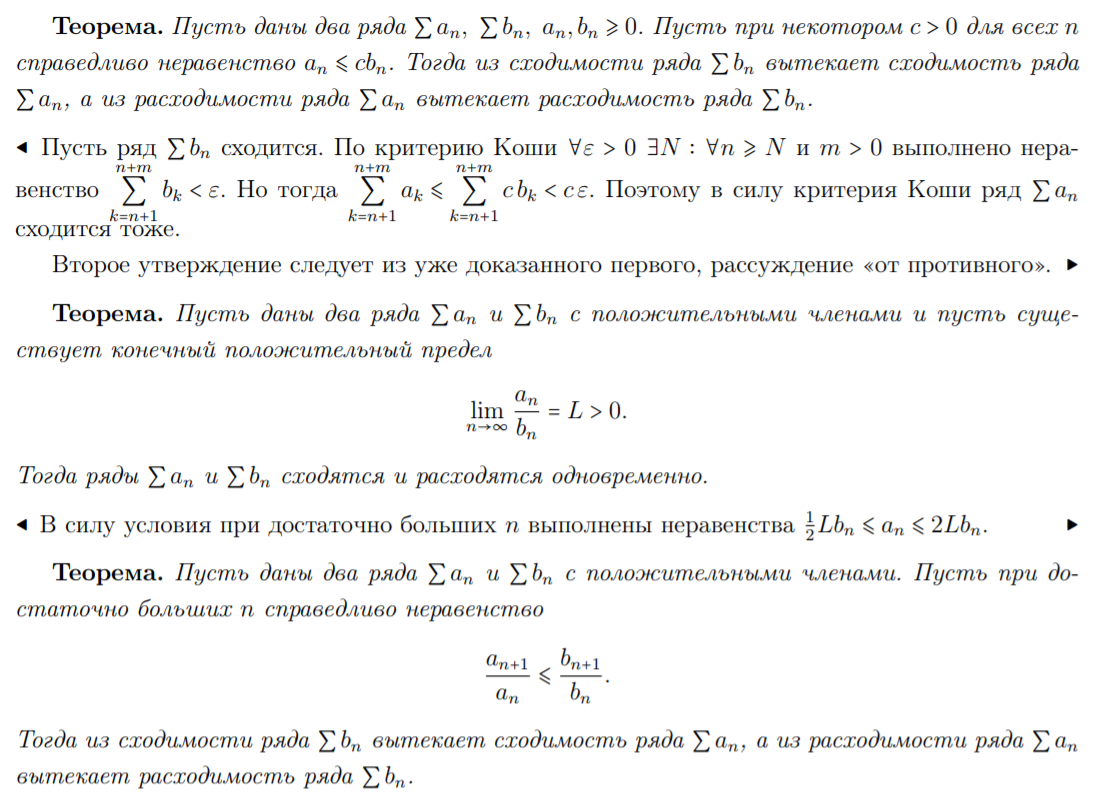
\includegraphics[scale=0.35]{Pictures/17_1.png}
\end{figure}
\begin{figure}[h!]
\centering
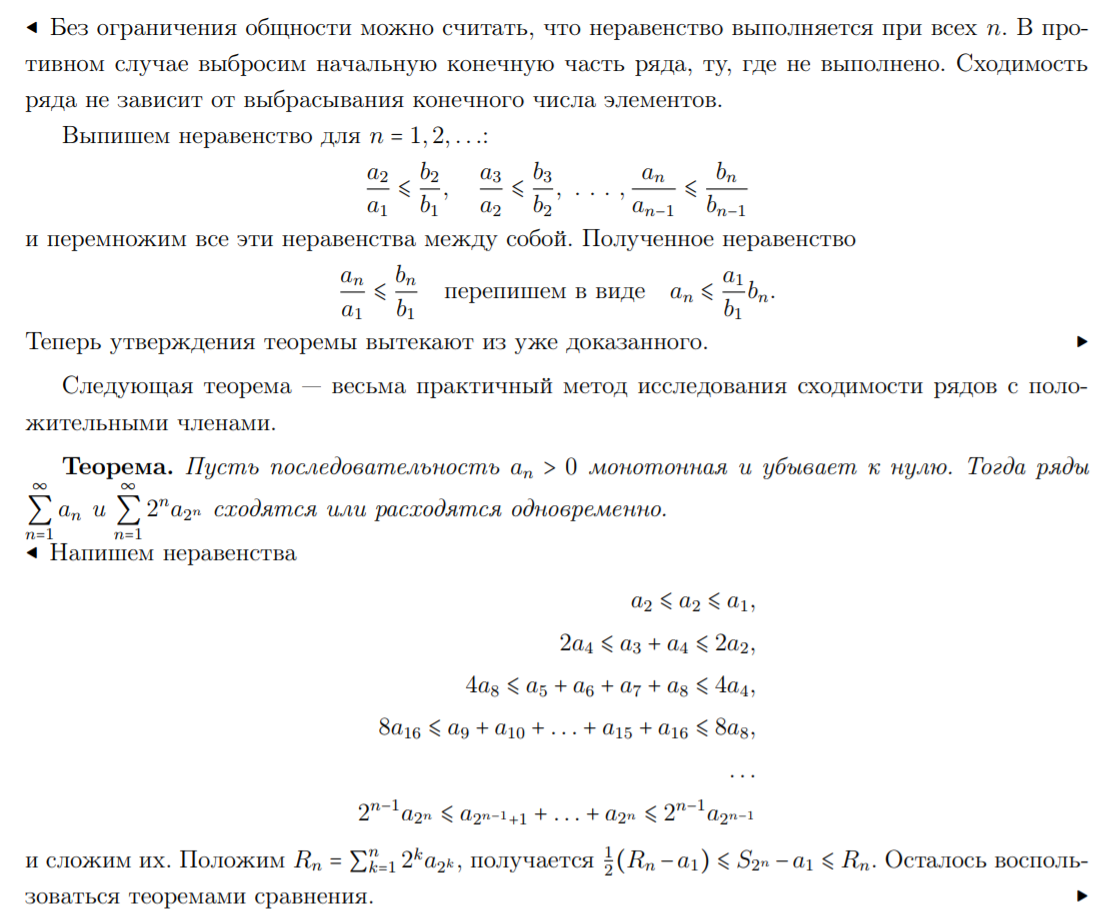
\includegraphics[scale=0.35]{Pictures/17_2.png}
\end{figure}
\newpage


%18 done
\section{Признак через $a_{2^n}$.}

\textbf{Телескопический признак:}
 
Для каждого такой монотонно убывающей последовательности $f(n)(n \in \mathbb{N})$, причем $\forall n \in \mathbb{N} f(n)\geqslant 0 $, тогда ряд $\sum_{n}^{\infty} f(2^n)$ сходится или расходится тогда и только тогда когда ряд $\Sum_{n}^{\infty} f(n)$ сходится или расходится соответственно.

\textit{Доказательство:}

\textit{Лемма:}
Заметим что $\forall k,n \{k>n\} \; (k-n)*f(n)\geqslant f(n+1)+f(n+2)+...+f(k)$, ввиду того что последовательность $f(n)$ убывающая.\\
\begin{align*}
\Sum_{n}^{\infty} f(n)=f(1)+f(2)+f(3)+...
\end{align*}
Распишем ряд следующим образом, для каждого такого элемента ряда $\Sum_{n}^{\infty} f(n)$, такого что $n=2^{k}$ распишем все последующие $2^{n}$ элементов ряда как $k*2^{n}$, тогда соответственно следующий ряд $f(1)*1+f(2)*2+f(4)*4+... \Leftrightarrow \Sum_{n}^{\infty} 2^n*f(2^n)$, причем в силлу леммы  $0<\Sum_{n}^{\infty} 2^n*f(2^n)\geqslant \Sum_{n}^{\infty} f(n) $, тогда по признаку сравнения рядов, если ряд $\Sum_{n}^{\infty} 2^n*f(2^n)$ сходится, тогда ряд $\Sum_{n}^{\infty} f(n)$ тем более сходится. Тоже утверждение следственно верно и для расходимости ввиду признака сравнения.

%19 done
\section{Признаки Даламбера и Коши.}

\underline{Признак Даламбера.}
\textit{Пусть $a_n > 0.$ Положим $\mathfrak{D}_n=\frac{a_{n+1}}{a_n}.$}\\
\textit{Если для всех достаточно больших $n$ справедливо неравенство $\mathfrak{D}_n \leq q < 1$, то ряд $\Sum a_n$ сходится. Если для всех достаточно больших $n$ справедливо неравенство $\mathfrak{D}_n \geq 1$, то ряд $\Sum a_n$ расходится.}\\
Пусть существует предел $\lim_{n \rightarrow \infty} \mathfrak{D}_n = d$. Если $d < 1,$ то ряд $\Sum a_n$ сходится; если $d > 1$, то ряд $\Sum a_n$ расходится (\textit{признак Даламбера в предельной форме.})\\

\underline{Признак Коши.}
\textit{Пусть $a_n > 0$, положим $\mathfrak{C}_n = \sqrt[3]{a_n}.$ Если при достаточно больших $n$ cправедливо неравенство $\mathfrak{C}_n \leq q < 1,$ то ряд $\sum a_n$ сходится. Если при бесконечном множестве достаточно больших $n$ справедливо неравенство $\mathfrak{C}_n \geq 1,$ то ряд $\sum a_n$ расходится.}  \\
$\blacktriangleleft$
В случае $\mathfrak{C}_n \leq q < 1$ сравним ряд $\sum a_n$ со сходящейся геометрической прогрессией $\sum q^n$, в случае $q > 1$ не выполнено необходимое условие сходимости. $\blacktriangleright$
\\

%20 done
\section{Число $e = \lim_{n \to\infty}{x_n}$ — существование предела.}

\underline{Бином Ньютона.}\\
$(a+b)^n = a^n + C_{n}^1 a^{n - 1} b + C_{n}^2 a{n - 2} b^2 + ... + b^n$ \\
\underline{Неравенство Бернулли.} Для всех $\alpha > -1$ и $n \in \bb{N}$ справедливо неравенство  \\
$(1 + \alpha)^n \geq 1 + n \alpha$ (доказательство по индукции) \\
 \begin{figure}[h!]
\centering
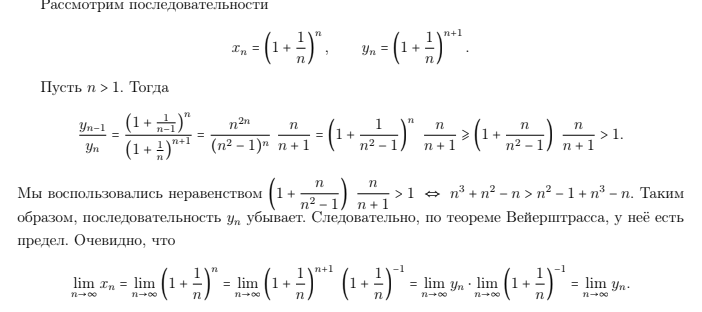
\includegraphics[scale=0.6]{Pictures/20_1.png}
\end{figure}
 \begin{figure}[h!]
\centering
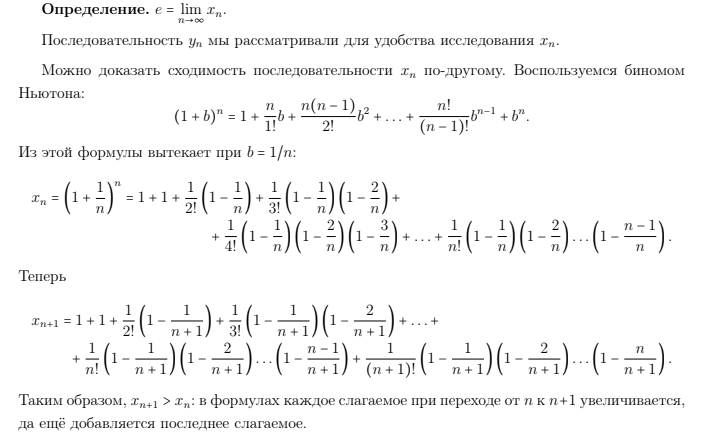
\includegraphics[scale=0.6]{Pictures/20_2.png}
\end{figure}
 \begin{figure}[h!]
\centering
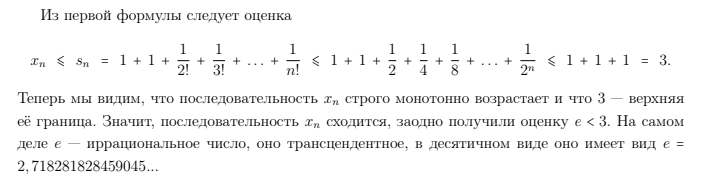
\includegraphics[scale=0.6]{Pictures/20_3.png}
\end{figure}
\newpage

%21 done
\section{Представление $e$ в виде суммы ряда из обратных факториалов. Иррациональность числа $e$.}

 \begin{figure}[h!]
\centering
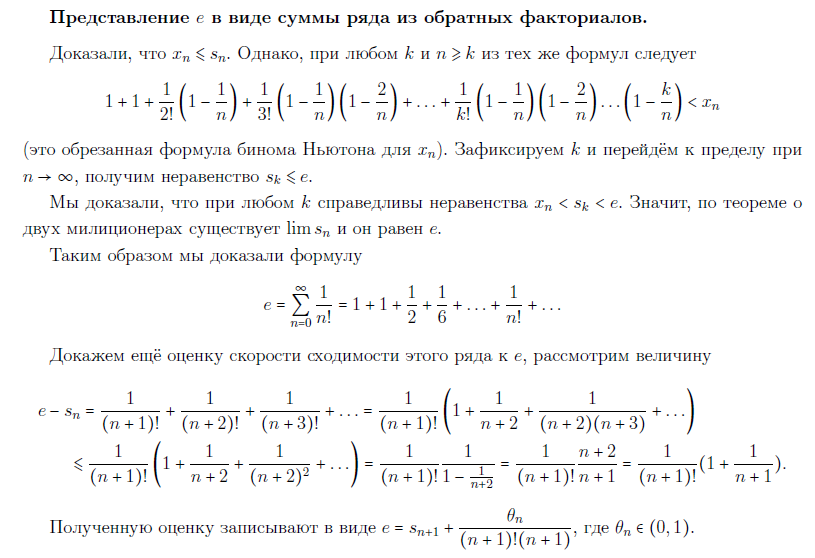
\includegraphics[scale=0.7]{Pictures/21_1.PNG}
\end{figure}
 \begin{figure}[h!]
\centering
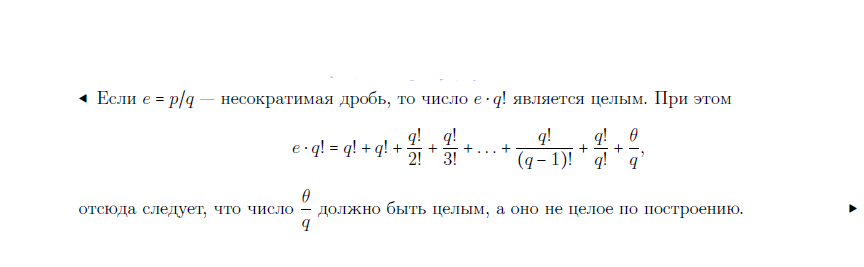
\includegraphics[scale=0.7]{Pictures/21_2.PNG}
\end{figure}
\newpage

%22 done
\section{Предел функции. Предел функции по Гейне.}

\textit{Проколотая окрестность точки $a$} -- это окрестность точки $a$ без точки $a$. Обозначение $O^{\circ}(a)$. 
 \begin{figure}[h!]
\centering
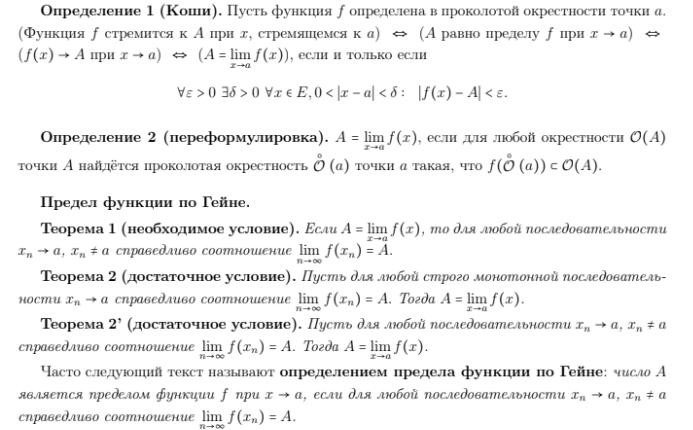
\includegraphics[scale=0.6]{Pictures/22_1.png}
\end{figure}
 \begin{figure}[h!]
\centering
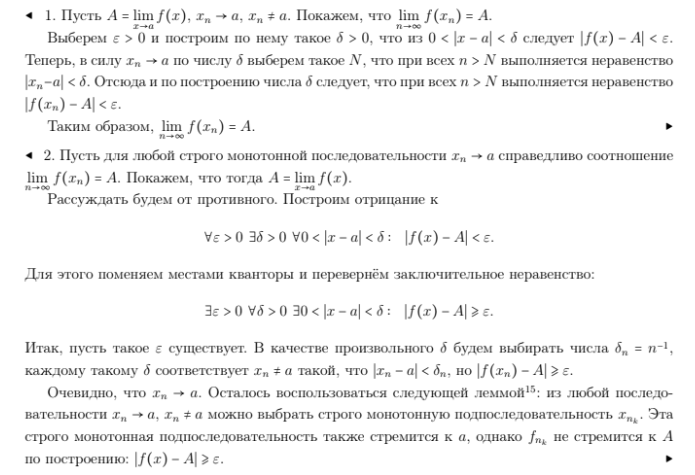
\includegraphics[scale=0.6]{Pictures/22_2.png}
\end{figure}
\newpage




%23 done
\section{Критерий Коши существования предела функции.}

 \begin{figure}[h!]
\centering
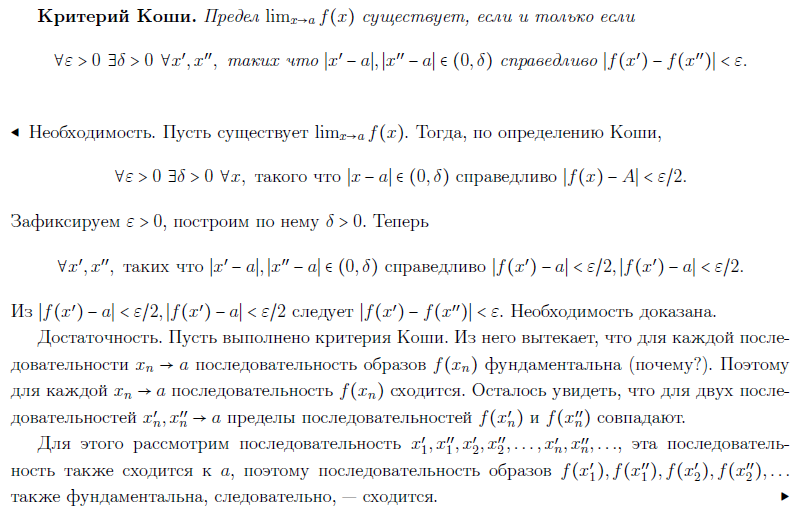
\includegraphics[scale=0.8]{Pictures/23.PNG}
\end{figure}



%24 done
\section{Первый замечательный предел.}

Первый замечательный предел: 
$\lim_{x \rightarrow 0} \frac{\sin{x}}{x} = 1$\\
 \begin{figure}[h!]
\centering
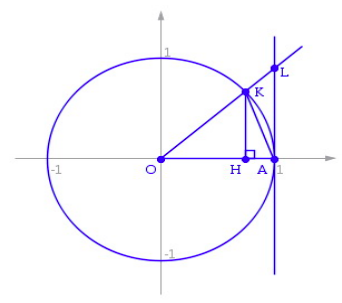
\includegraphics[scale=0.7]{Pictures/24_1.png}
\end{figure}
 \begin{figure}[h!]
\centering
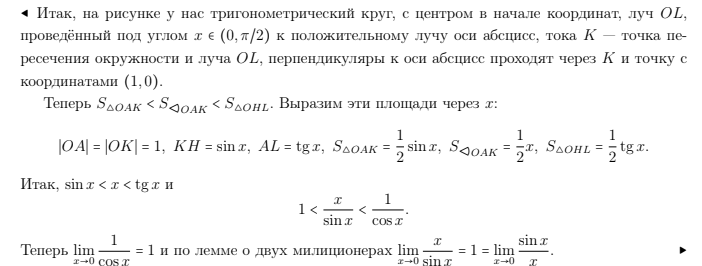
\includegraphics[scale=0.7]{Pictures/24_2.png}
\end{figure}

%25 done
\section{Второй замечательный предел.}

$\lim_{t \rightarrow} (1 + t)^{1/t} = \lim_{x \rightarrow \infty} (1 + \frac{1}{x})^x = e$
 \begin{figure}[h!]
\centering
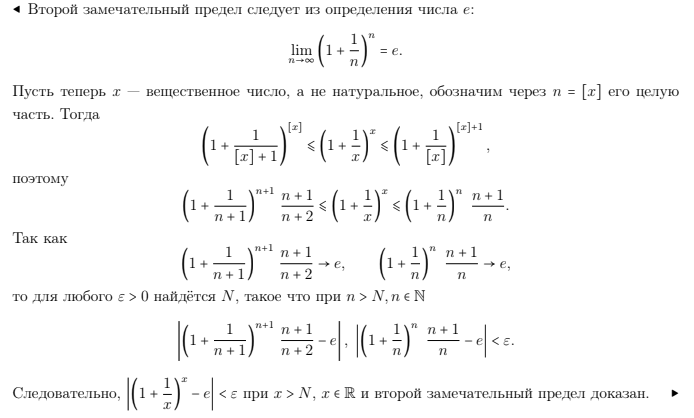
\includegraphics[scale=0.7]{Pictures/25.png}
\end{figure}
\newpage

%26 done
\section{Предел сложной функции. Замена переменных в пределах.}

\begin{figure}[h!]
\centering
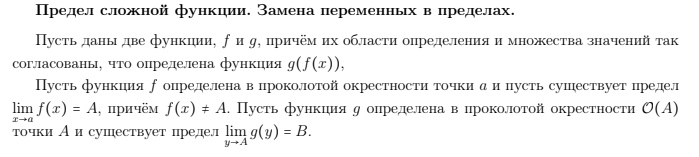
\includegraphics[scale=0.7]{Pictures/26_1.png}
\end{figure}
 \begin{figure}[h!]
\centering
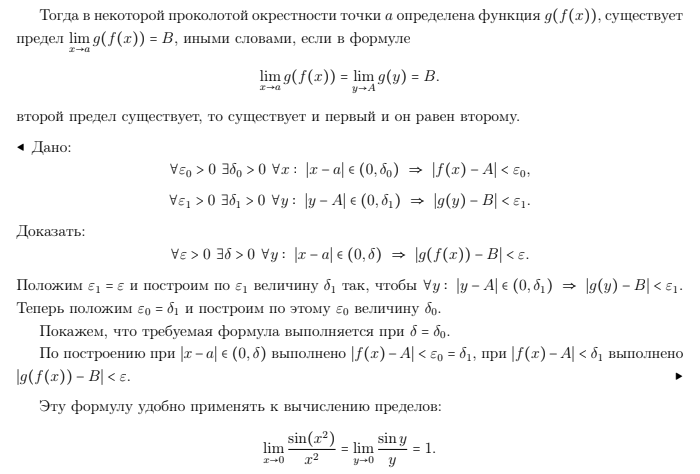
\includegraphics[scale=0.7]{Pictures/26_2.png}
\end{figure}
\newpage

%27 done
\section{Односторонние пределы — определение, примеры. Существование односторонних пределов у монотонной функции.}

 \begin{figure}[h!]
\centering
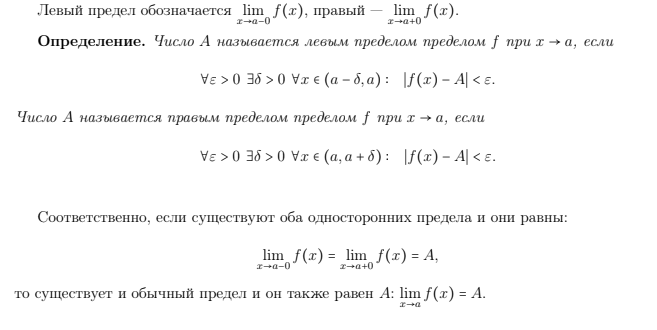
\includegraphics[scale=0.65]{Pictures/27_1.png}
\end{figure}
 \begin{figure}[h!]
\centering
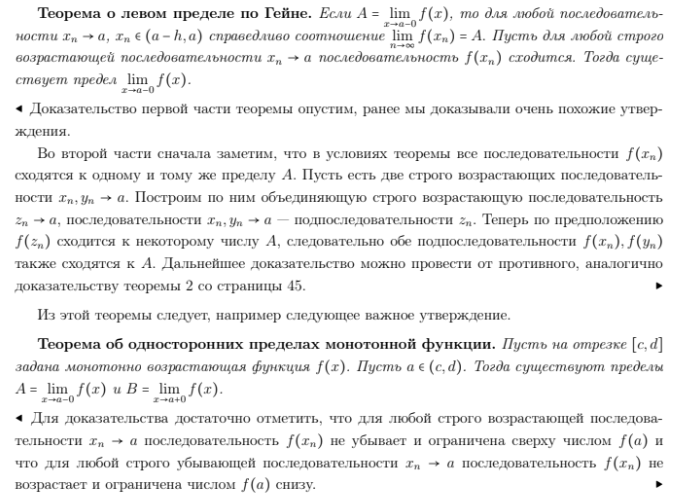
\includegraphics[scale=0.65]{Pictures/27_2.png}
\end{figure}
\newpage

%28 done
\section{Непрерывные функции. Разрывы, классификация точек разрыва.Примеры}

\begin{figure}[h!]
\centering
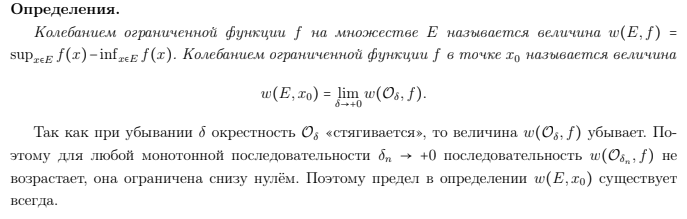
\includegraphics[scale=0.6]{Pictures/28_1.png}
\end{figure}
 \begin{figure}[h!]
\centering
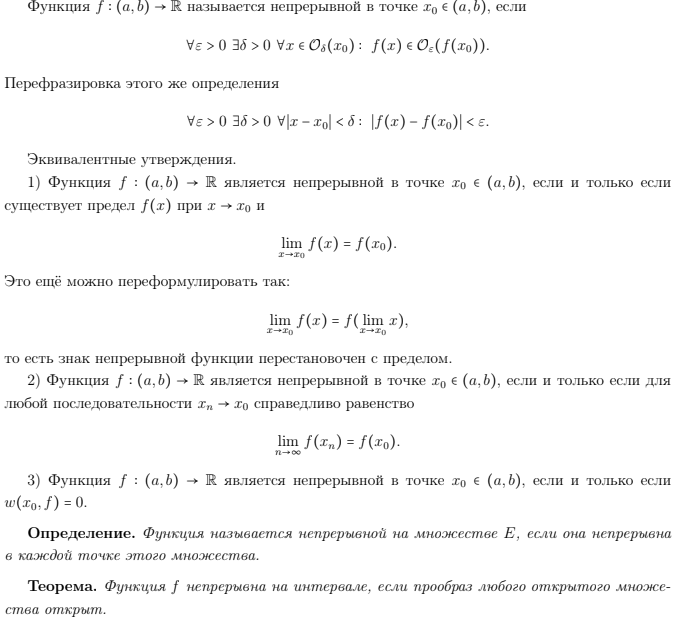
\includegraphics[scale=0.65]{Pictures/28_2.png}
\end{figure}
\begin{figure}[h!]
\centering
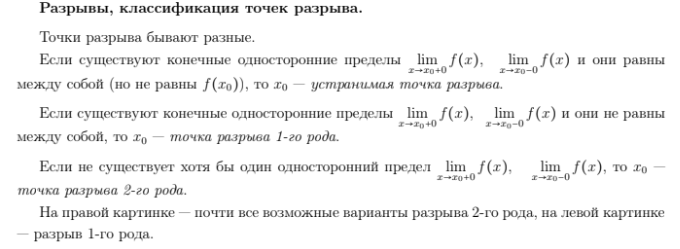
\includegraphics[scale=0.65]{Pictures/28_3.png}
\end{figure}
\newpage

%29 done
\section{}

\textbf{Локальные свойства непрерывных функций.Теорема о непрерывности сложной функции.}
 \begin{figure}[h!]
\centering
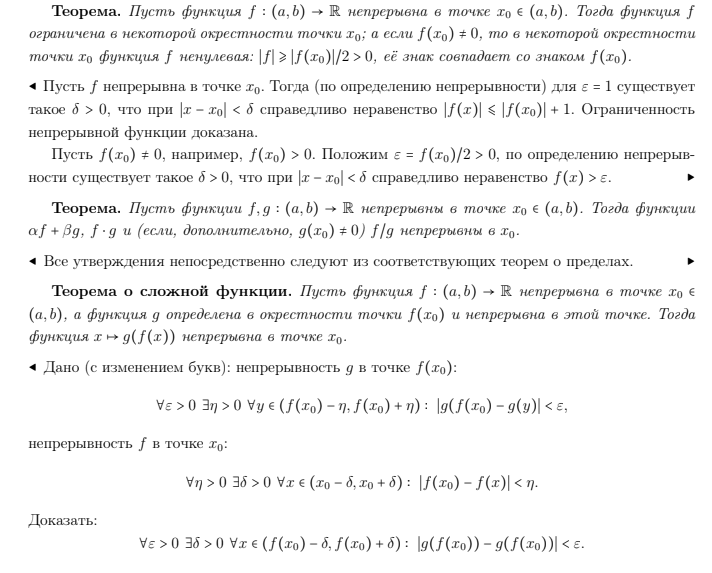
\includegraphics[scale=0.6]{Pictures/29_1.png}
\end{figure}
\begin{figure}[h!]
\centering
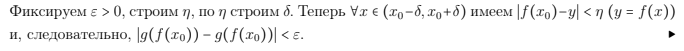
\includegraphics[scale=0.6]{Pictures/29-2.png}
\end{figure}
\newpage

%30
\section{}

\textbf{Глобальные свойства непрерывных функций. Ограниченность, максимум ограниченной функции достигается.}
\begin{figure}[h!]
\centering
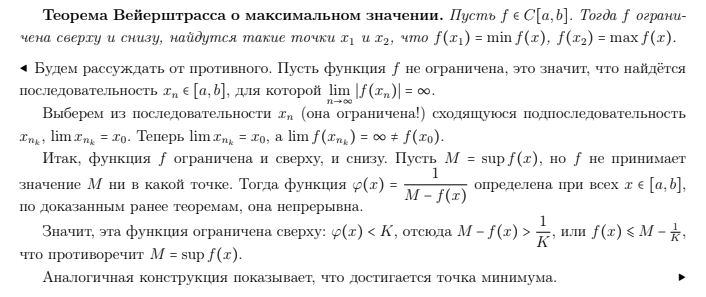
\includegraphics[scale=0.7]{Pictures/30.png}
\end{figure}




%31 done
\section{Глобальные свойства непрерывных функций. Теорема о промежуточном значении.}

\begin{figure}[h!]
\centering
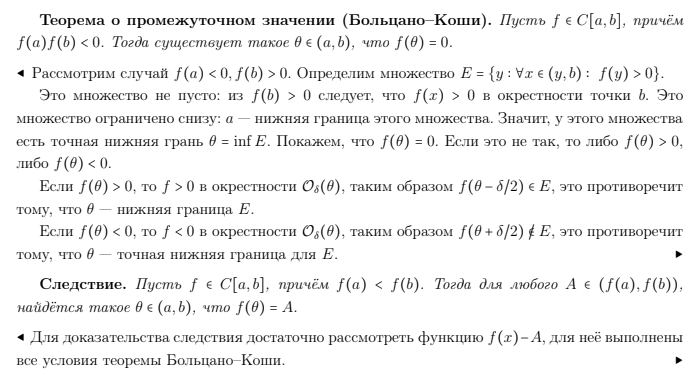
\includegraphics[scale=0.7]{Pictures/31.png}
\end{figure}
\newpage


%32 done
\section{Глобальные свойства непрерывных функций. Непрерывный образ отрезка -- отрезок.}

 \begin{figure}[h!]
\centering
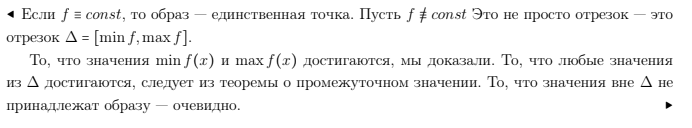
\includegraphics[scale=0.7]{Pictures/32.png}
\end{figure}


%33 done
\section{Глобальные свойства непрерывных функций. Равномерная непрерывность, теорема Кантора.}
 
 \begin{figure}[h!]
\centering
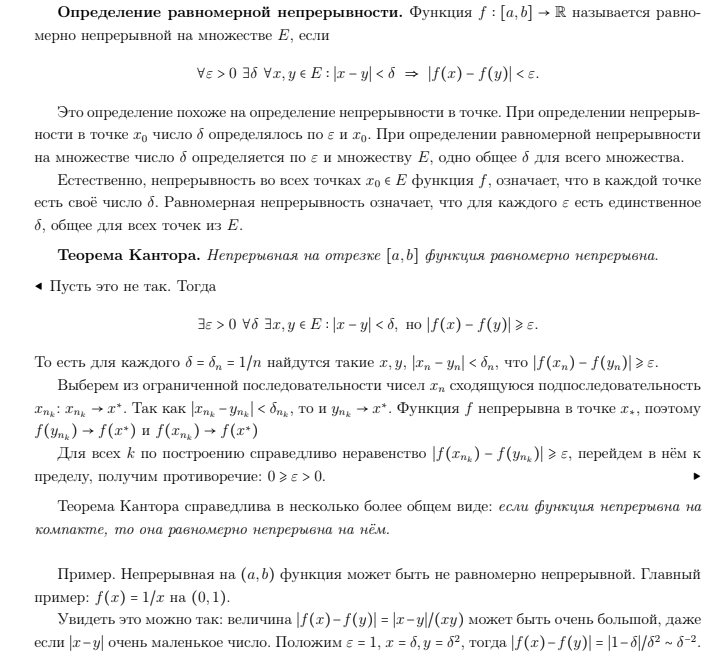
\includegraphics[scale=0.6]{Pictures/33.png}
\end{figure}

